% ==============================================================================
% CHAPTER 8: INFORMATION THEORY AND LOSS FUNCTIONS
% ==============================================================================

\chapter{Information Theory and Loss Functions}
\label{ch:information_theory}

\begin{keyconcept}
Information theory provides the mathematical foundation for understanding how to measure the ``distance'' between probability distributions. This leads to principled loss functions like \textbf{cross-entropy}, which are fundamental to training neural networks for classification.
\end{keyconcept}

% ------------------------------------------------------------------------------
\section{The Learning Problem}
% ------------------------------------------------------------------------------

\subsection{Setup}

We have:
\begin{itemize}
    \item An unknown true function $g: \mathcal{X} \to \mathcal{Y}$
    \item A dataset $\mathcal{D} = \{(x_i, y_i)\}_{i=1}^N$ sampled from some distribution
    \item A model $f_\theta$ parameterized by $\theta$
    \item Goal: Find $\theta$ such that $f_\theta(x) \approx g(x)$ for all $x$
\end{itemize}

\subsection{The Divergence Problem}

To measure how well our model $f_\theta$ approximates the true function $g$, we need a \textbf{divergence function}:
\[
D(f_\theta, g): \text{measures ``distance'' between } f_\theta \text{ and } g
\]

\textbf{Problem}: We don't know $g$! We only have samples $(x, y)$ from it.

\textbf{Solution}: We use the \textbf{empirical distribution} from our data as a proxy for the true distribution.

% ------------------------------------------------------------------------------
\section{Information and Surprise}
% ------------------------------------------------------------------------------

\subsection{Intuition: Data as Surprise}

\begin{infobox}{The Core Insight}
When we receive data, we gain \textbf{information}. Information is inversely related to \textbf{probability}---the less likely an event, the more surprising (informative) it is when it occurs.
\end{infobox}

Consider tossing a fair coin:
\begin{itemize}
    \item Getting heads has probability $\frac{1}{2}$
    \item Getting heads 10 times in a row has probability $\left(\frac{1}{2}\right)^{10} = \frac{1}{1024}$
\end{itemize}
The second event is much more ``surprising'' and thus carries more information.

\subsection{Defining Information}

We want a function $I(p)$ that measures the ``information content'' of an event with probability $p$:

\textbf{Desirable Properties:}
\begin{enumerate}
    \item $I(1) = 0$ (certain events provide no information)
    \item $I(p)$ should be decreasing in $p$ (rare events are more informative)
    \item $I(p_1 \cdot p_2) = I(p_1) + I(p_2)$ (information from independent events should add)
\end{enumerate}

\begin{derivation}{Information Content}
From property 3, we need $I(p_1 \cdot p_2) = I(p_1) + I(p_2)$.

The logarithm is the only function satisfying this:
\[
\log(p_1 \cdot p_2) = \log(p_1) + \log(p_2)
\]

But $\log(p)$ is negative for $p < 1$, and we want positive information. So:
\[
\boxed{I(p) = -\log(p) = \log\left(\frac{1}{p}\right)}
\]

For base 2, information is measured in \textbf{bits}.
\end{derivation}

\textbf{Examples:}
\begin{itemize}
    \item Fair coin flip: $I(0.5) = -\log_2(0.5) = 1$ bit
    \item Rolling a 6 on a fair die: $I(1/6) = -\log_2(1/6) \approx 2.58$ bits
    \item Rolling 10 sixes in a row: $I((1/6)^{10}) \approx 25.8$ bits
\end{itemize}

% ------------------------------------------------------------------------------
\section{Entropy}
% ------------------------------------------------------------------------------

\subsection{Definition}

\textbf{Entropy} measures the \textit{expected} (average) information content of a random variable.

\begin{definition}[Entropy]
For a discrete random variable $X$ with probability distribution $P(X)$:
\[
\boxed{H(X) = -\sum_{x} P(x) \log P(x) = \mathbb{E}_{x \sim P}[-\log P(x)]}
\]
\end{definition}

This is the \textbf{expected surprise} when observing samples from distribution $P$.

\subsection{Properties of Entropy}

\begin{itemize}
    \item $H(X) \geq 0$ (entropy is non-negative)
    \item $H(X) = 0$ if and only if $X$ is deterministic (one outcome has probability 1)
    \item For $n$ equally likely outcomes: $H(X) = \log n$ (maximum entropy)
\end{itemize}

\subsection{Examples}

\textbf{Fair coin ($p = 0.5$):}
\begin{align}
H &= -[0.5 \log_2(0.5) + 0.5 \log_2(0.5)] \\
&= -[0.5 \cdot (-1) + 0.5 \cdot (-1)] = 1 \text{ bit}
\end{align}

\textbf{Biased coin ($p = 0.9$ for heads):}
\begin{align}
H &= -[0.9 \log_2(0.9) + 0.1 \log_2(0.1)] \\
&\approx -[0.9 \cdot (-0.152) + 0.1 \cdot (-3.322)] \\
&\approx 0.469 \text{ bits}
\end{align}

\begin{important}
The biased coin has \textbf{lower entropy}---its outcomes are more predictable!
\end{important}

\subsection{Entropy Visualization}

For a binary random variable with $P(\text{heads}) = p$:
\[
H(p) = -p\log_2(p) - (1-p)\log_2(1-p)
\]

\begin{center}
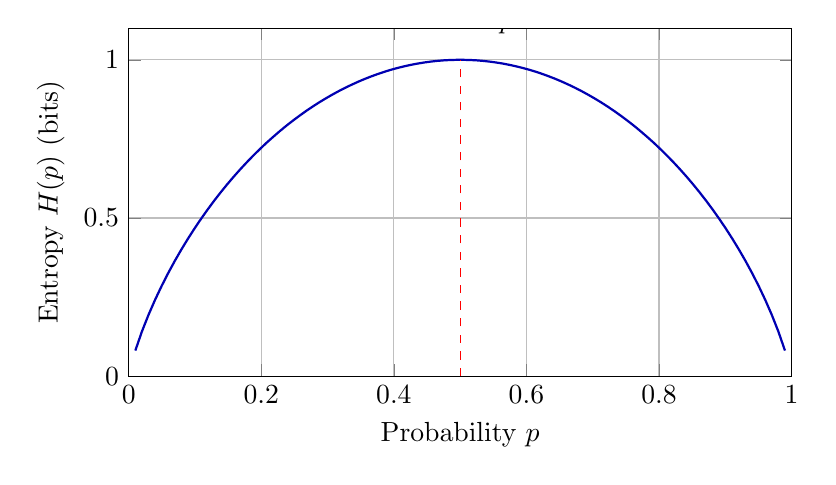
\begin{tikzpicture}
\begin{axis}[
    width=10cm,
    height=6cm,
    xlabel={Probability $p$},
    ylabel={Entropy $H(p)$ (bits)},
    xmin=0, xmax=1,
    ymin=0, ymax=1.1,
    grid=both,
    samples=100,
    domain=0.01:0.99,
]
\addplot[thick, blue!70!black] {-x*ln(x)/ln(2) - (1-x)*ln(1-x)/ln(2)};
\addplot[dashed, red] coordinates {(0.5, 0) (0.5, 1)};
\node at (axis cs:0.5,1.05) [anchor=south] {Maximum at $p=0.5$};
\end{axis}
\end{tikzpicture}
\end{center}

% ------------------------------------------------------------------------------
\section{Cross-Entropy}
% ------------------------------------------------------------------------------

\subsection{Motivation}

Suppose we have:
\begin{itemize}
    \item True distribution $P$ (the actual data distribution)
    \item Approximate distribution $Q$ (our model's predictions)
\end{itemize}

\textbf{Cross-entropy} measures the expected information content when we use distribution $Q$ to encode events that actually come from distribution $P$.

\begin{definition}[Cross-Entropy]
\[
\boxed{H(P, Q) = -\sum_{x} P(x) \log Q(x) = \mathbb{E}_{x \sim P}[-\log Q(x)]}
\]
\end{definition}

\textbf{Interpretation}: If the true distribution is $P$ but we encode using $Q$, cross-entropy tells us the average number of bits needed per message.

\subsection{Key Insight}

\begin{theorem}[Cross-Entropy and Entropy]
\[
H(P, Q) \geq H(P)
\]
with equality if and only if $Q = P$.
\end{theorem}

This tells us:
\begin{itemize}
    \item Using the wrong distribution $Q \neq P$ always requires more bits on average
    \item Cross-entropy is minimized when $Q = P$
    \item Therefore, minimizing cross-entropy pushes $Q$ toward $P$!
\end{itemize}

% ------------------------------------------------------------------------------
\section{KL Divergence}
% ------------------------------------------------------------------------------

\subsection{Definition}

The \textbf{Kullback-Leibler (KL) divergence} measures the ``extra bits'' needed when using $Q$ instead of $P$:

\begin{definition}[KL Divergence]
\[
\boxed{D_{KL}(P \| Q) = \sum_{x} P(x) \log \frac{P(x)}{Q(x)} = H(P, Q) - H(P)}
\]
\end{definition}

\textbf{Interpretation}: KL divergence is the ``waste'' in using $Q$ to encode data from $P$.

\subsection{Properties}

\begin{itemize}
    \item $D_{KL}(P \| Q) \geq 0$ (Gibbs' inequality)
    \item $D_{KL}(P \| Q) = 0$ if and only if $P = Q$
    \item \textbf{Not symmetric}: $D_{KL}(P \| Q) \neq D_{KL}(Q \| P)$ in general
    \item Not a true metric (doesn't satisfy triangle inequality)
\end{itemize}

\subsection{Why Cross-Entropy for Loss?}

In minimizing loss, we want $Q_{\theta}$ (our model) to match $P$ (true distribution):
\[
\min_\theta D_{KL}(P \| Q_\theta) = \min_\theta \left[ H(P, Q_\theta) - H(P) \right]
\]

Since $H(P)$ doesn't depend on $\theta$:
\[
\min_\theta D_{KL}(P \| Q_\theta) = \min_\theta H(P, Q_\theta)
\]

\begin{important}
\textbf{Minimizing cross-entropy is equivalent to minimizing KL divergence!}

This is why cross-entropy is the natural loss function for classification.
\end{important}

% ------------------------------------------------------------------------------
\section{The Softmax Function}
% ------------------------------------------------------------------------------

For multi-class classification, we need to convert network outputs into a probability distribution. The \textbf{softmax function} accomplishes this.

\begin{definition}[Softmax]
For a vector $z = (z_1, z_2, \ldots, z_K)$ of logits:
\[
\boxed{\text{softmax}(z)_i = \frac{e^{z_i}}{\sum_{j=1}^{K} e^{z_j}}}
\]
\end{definition}

\subsection{Properties}

\begin{enumerate}
    \item \textbf{Valid probability distribution}: All outputs are positive and sum to 1
    \[
    \sum_{i=1}^{K} \text{softmax}(z)_i = 1
    \]
    
    \item \textbf{Preserves ordering}: If $z_i > z_j$, then $\text{softmax}(z)_i > \text{softmax}(z)_j$
    
    \item \textbf{Differentiable}: Can be used with gradient-based optimization
    
    \item \textbf{Shift invariance}: $\text{softmax}(z + c) = \text{softmax}(z)$ for any constant $c$
\end{enumerate}

\subsection{Example}

For $z = (2, 1, 0)$:
\begin{align}
\text{softmax}(z) &= \frac{1}{e^2 + e^1 + e^0}(e^2, e^1, e^0) \\
&= \frac{1}{7.389 + 2.718 + 1}(7.389, 2.718, 1) \\
&\approx (0.665, 0.245, 0.090)
\end{align}

\subsection{Softmax Temperature}

A generalization introduces \textbf{temperature} $T$:
\[
\text{softmax}(z/T)_i = \frac{e^{z_i/T}}{\sum_{j} e^{z_j/T}}
\]

\begin{itemize}
    \item $T \to 0$: Outputs become one-hot (winner-take-all)
    \item $T = 1$: Standard softmax
    \item $T \to \infty$: Outputs become uniform
\end{itemize}

% ------------------------------------------------------------------------------
\section{Cross-Entropy Loss for Classification}
% ------------------------------------------------------------------------------

\subsection{Binary Classification: Binary Cross-Entropy (BCE)}

For binary classification with true label $y \in \{0, 1\}$ and predicted probability $\hat{y} = P(Y=1|X)$:

\begin{definition}[Binary Cross-Entropy Loss]
\[
\boxed{\mathcal{L}_{BCE} = -[y \log(\hat{y}) + (1-y) \log(1 - \hat{y})]}
\]
\end{definition}

\textbf{Analysis by cases:}
\begin{itemize}
    \item If $y = 1$: $\mathcal{L} = -\log(\hat{y})$ (penalizes low $\hat{y}$)
    \item If $y = 0$: $\mathcal{L} = -\log(1 - \hat{y})$ (penalizes high $\hat{y}$)
\end{itemize}

\subsection{Multi-class Classification: Categorical Cross-Entropy (CCE)}

For $K$ classes with one-hot encoded true label $y = (y_1, \ldots, y_K)$ and predicted probabilities $\hat{y} = (\hat{y}_1, \ldots, \hat{y}_K)$:

\begin{definition}[Categorical Cross-Entropy Loss]
\[
\boxed{\mathcal{L}_{CCE} = -\sum_{k=1}^{K} y_k \log(\hat{y}_k)}
\]

Since $y$ is one-hot (only one $y_c = 1$, others are 0):
\[
\mathcal{L}_{CCE} = -\log(\hat{y}_c)
\]
where $c$ is the true class.
\end{definition}

\textbf{Interpretation}: We only penalize the predicted probability of the \textit{correct} class.

\subsection{Example: Multi-class Classification}

\textbf{Scenario}: 3-class classification, true class is 2.

True label (one-hot): $y = (0, 1, 0)$

Predicted probabilities: $\hat{y} = (0.1, 0.7, 0.2)$

\[
\mathcal{L} = -[\underbrace{0 \cdot \log(0.1)}_{=0} + \underbrace{1 \cdot \log(0.7)}_{=-0.357} + \underbrace{0 \cdot \log(0.2)}_{=0}] = 0.357
\]

If prediction were perfect ($\hat{y} = (0, 1, 0)$): $\mathcal{L} = -\log(1) = 0$.

% ------------------------------------------------------------------------------
\section{Maximum Likelihood Estimation Perspective}
% ------------------------------------------------------------------------------

Cross-entropy loss emerges naturally from the \textbf{maximum likelihood estimation} (MLE) framework.

\subsection{The Four-Step Recipe for Loss Construction}

\begin{algorithm}[Constructing Loss Functions via MLE]
\begin{enumerate}
    \item \textbf{Choose a probability distribution} for the output $Y$
    \item \textbf{Parameterize the distribution} with the neural network output
    \item \textbf{Compute negative log-likelihood} (this is your loss)
    \item \textbf{Find argmax} for inference (point prediction)
\end{enumerate}
\end{algorithm}

\subsection{Deriving Binary Cross-Entropy}

\textbf{Step 1}: Model output as Bernoulli distribution
\[
P(Y = y | X = x) = \hat{y}^y (1 - \hat{y})^{1-y}
\]
where $\hat{y} = \sigma(\theta^\top x)$ (sigmoid output).

\textbf{Step 2}: Likelihood for $N$ i.i.d. samples
\[
\mathcal{L}(\theta) = \prod_{i=1}^{N} P(y_i | x_i; \theta) = \prod_{i=1}^{N} \hat{y}_i^{y_i}(1-\hat{y}_i)^{1-y_i}
\]

\textbf{Step 3}: Negative log-likelihood
\begin{align}
-\log \mathcal{L}(\theta) &= -\sum_{i=1}^{N} \left[ y_i \log \hat{y}_i + (1-y_i)\log(1-\hat{y}_i) \right] \\
&= \sum_{i=1}^{N} \mathcal{L}_{BCE}(y_i, \hat{y}_i)
\end{align}

\begin{important}
Binary cross-entropy is simply the negative log-likelihood of the Bernoulli distribution!
\end{important}

\subsection{Deriving Categorical Cross-Entropy}

\textbf{Step 1}: Model output as Categorical distribution
\[
P(Y = k | X) = \hat{y}_k = \text{softmax}(z)_k
\]

\textbf{Step 2}: Likelihood (one-hot representation)
\[
P(Y = y | X) = \prod_{k=1}^{K} \hat{y}_k^{y_k}
\]

\textbf{Step 3}: Negative log-likelihood
\[
-\log P(Y = y | X) = -\sum_{k=1}^{K} y_k \log \hat{y}_k = \mathcal{L}_{CCE}
\]

\subsection{MSE from Gaussian Assumption}

\textbf{Step 1}: Assume Gaussian noise
\[
P(y | x) = \mathcal{N}(y | \hat{y}, \sigma^2)
\]

\textbf{Step 2}: Negative log-likelihood
\begin{align}
-\log P(y | x) &= -\log\left[\frac{1}{\sqrt{2\pi\sigma^2}} \exp\left(-\frac{(y-\hat{y})^2}{2\sigma^2}\right)\right] \\
&= \frac{(y - \hat{y})^2}{2\sigma^2} + \text{const}
\end{align}

\begin{important}
Mean Squared Error is the negative log-likelihood of a Gaussian distribution!
\end{important}

% ------------------------------------------------------------------------------
\section{Gradient of Cross-Entropy with Softmax}
% ------------------------------------------------------------------------------

A remarkable property emerges when combining softmax with cross-entropy loss.

\begin{derivation}{Softmax + Cross-Entropy Gradient}
Let $z$ be the logits (pre-softmax), $\hat{y} = \text{softmax}(z)$, and $\mathcal{L} = -\sum_k y_k \log \hat{y}_k$.

For the gradient $\frac{\partial \mathcal{L}}{\partial z_i}$:

\textbf{Case 1}: $i = c$ (correct class)
\[
\frac{\partial \mathcal{L}}{\partial z_c} = \hat{y}_c - 1
\]

\textbf{Case 2}: $i \neq c$
\[
\frac{\partial \mathcal{L}}{\partial z_i} = \hat{y}_i
\]

\textbf{Combined (vector form)}:
\[
\boxed{\frac{\partial \mathcal{L}}{\partial z} = \hat{y} - y}
\]
\end{derivation}

This is remarkably simple! The gradient is just the difference between predicted and true probabilities.

% ------------------------------------------------------------------------------
\section{Why Use Logarithms?}
% ------------------------------------------------------------------------------

Several practical reasons favor log-probabilities:

\begin{enumerate}
    \item \textbf{Numerical stability}: Products of probabilities become tiny; logs convert to sums
    \[
    \log(p_1 \cdot p_2 \cdots p_n) = \log p_1 + \log p_2 + \cdots + \log p_n
    \]
    
    \item \textbf{Underflow prevention}: $10^{-300} \cdot 10^{-300}$ underflows to 0, but $-300 + (-300) = -600$ is fine
    
    \item \textbf{Convexity}: Log-likelihood often has nicer optimization landscapes
    
    \item \textbf{Interpretability}: Log-probabilities have units of ``bits'' or ``nats''
\end{enumerate}

% ------------------------------------------------------------------------------
\section{Summary: Loss Function Selection}
% ------------------------------------------------------------------------------

\begin{summary}
\textbf{The Big Picture:}
\begin{itemize}
    \item Information theory provides principled foundations for loss functions
    \item Cross-entropy measures how well our predictions match the true distribution
    \item Minimizing cross-entropy = minimizing KL divergence = maximum likelihood estimation
\end{itemize}

\textbf{Loss Function Selection:}
\begin{center}
\begin{tabular}{lll}
\toprule
\textbf{Task} & \textbf{Assumption} & \textbf{Loss Function} \\
\midrule
Binary Classification & Bernoulli & Binary Cross-Entropy \\
Multi-class Classification & Categorical & Categorical Cross-Entropy \\
Regression & Gaussian noise & Mean Squared Error \\
\bottomrule
\end{tabular}
\end{center}

\textbf{Key Equations:}
\begin{align}
H(P) &= -\sum_x P(x) \log P(x) && \text{Entropy} \\[0.5em]
H(P, Q) &= -\sum_x P(x) \log Q(x) && \text{Cross-Entropy} \\[0.5em]
D_{KL}(P \| Q) &= H(P, Q) - H(P) && \text{KL Divergence} \\[0.5em]
\mathcal{L}_{BCE} &= -[y \log \hat{y} + (1-y)\log(1-\hat{y})] && \text{Binary CE} \\[0.5em]
\mathcal{L}_{CCE} &= -\sum_k y_k \log \hat{y}_k && \text{Categorical CE}
\end{align}
\end{summary}

% ------------------------------------------------------------------------------
\section{Practical Considerations}
% ------------------------------------------------------------------------------

\subsection{Label Smoothing}

Instead of hard one-hot labels, use soft labels:
\[
y_{\text{smooth}} = (1 - \epsilon) \cdot y + \frac{\epsilon}{K}
\]

This prevents overconfident predictions and improves generalization.

\subsection{Numerical Stability}

When computing $\log(\text{softmax}(z))$, use the numerically stable form:
\[
\log \text{softmax}(z)_i = z_i - \log\sum_j e^{z_j}
\]

Frameworks like PyTorch provide \texttt{log\_softmax} and \texttt{CrossEntropyLoss} that handle this automatically.
